\documentclass[10pt]{article}
\usepackage[margin=2.2cm]{geometry}
\usepackage{amsmath,amssymb,booktabs,graphicx,caption,longtable,url,hyperref}
\hypersetup{hidelinks}
\graphicspath{{../figures/}{figures/}}
\setlength{\emergencystretch}{2em}
\captionsetup{font=small}
\begin{document}
\begin{center}
{\Large\bfseries Supplementary Material}\\[4pt]
{\large\bfseries Measured Effects and Limits of Inference-Time Geometry-Adapter Scaling for Multi-view Texture Generation}
\end{center}

\section{S1. FRESH\_CONFIRM\_B generic schedule comparisons}

The generic schedule extension was executed on the same 150-object B cohort after the original analysis had been opened. It passed its 1,200/1,200-row integrity gate, but is a same-cohort post-lock sensitivity and not an independent confirmation. Each entry is LLH minus the comparator. Positive FG-PSNR and negative FG-LPIPS favor LLH. Holm correction is separate across the eight schedule comparisons for each metric.

\begin{table}[h]
\centering\scriptsize
\caption{Endpoint-specific generic schedule comparisons. Intervals are paired object-bootstrap 95\% CIs.}
\begin{tabular}{lrr}
\toprule
Schedule & FG-PSNR $\Delta$ [95\% CI]; Holm $p$ & FG-LPIPS $\Delta$ [95\% CI]; Holm $p$ \\
\midrule
Generic linear & -0.0373 [-0.0829, 0.0086]; 0.1150 & +0.0011 [0.0004, 0.0019]; 0.0024 \\
Linear, requested-mean matched & +0.0967 [0.0594, 0.1357]; $\leq$0.0008 & -0.0009 [-0.0013, -0.0004]; 0.0008 \\
Cosine bump & +0.3367 [0.2216, 0.4576]; $\leq$0.0008 & -0.0047 [-0.0059, -0.0034]; $\leq$0.0008 \\
Cosine bump, requested-mean matched & +0.4629 [0.3526, 0.5780]; $\leq$0.0008 & -0.0059 [-0.0071, -0.0046]; $\leq$0.0008 \\
Trapezoid & +0.1875 [0.0697, 0.3099]; 0.0036 & -0.0035 [-0.0047, -0.0023]; $\leq$0.0008 \\
Trapezoid, requested-mean matched & +0.4404 [0.3334, 0.5521]; $\leq$0.0008 & -0.0057 [-0.0070, -0.0045]; $\leq$0.0008 \\
Gaussian peak & +0.4092 [0.2934, 0.5302]; $\leq$0.0008 & -0.0052 [-0.0065, -0.0040]; $\leq$0.0008 \\
Gaussian peak, requested-mean matched & +0.4711 [0.3584, 0.5892]; $\leq$0.0008 & -0.0058 [-0.0071, -0.0045]; $\leq$0.0008 \\
\bottomrule
\end{tabular}
\end{table}

Requested-mean matching does not equalize measured correction norms. The nine-method total-dose central-90\% intersection is empty. Pairwise dose-conditioned models added after outcome exposure were underpowered or had insufficient overlap; they do not identify a dose-adjusted schedule-shape advantage. The complete condition-level cap and dose accounting is provided in \texttt{evidence/audits/FINAL\_CAP\_BUDGET\_CAUSAL\_ACCOUNTING.md} and \texttt{evidence/audits/FINAL\_GENERIC\_SCHEDULE\_COMPARISON.md}.

\section{S2. Multi-seed realization sensitivity}

E1 averages each object's paired effect over fixed generation seeds 42, 43, and 44 before object-level inference. Forty-eight objects were reused from B. The rows below show the LLH--LFM-exact comparison.

\begin{table}[h]
\centering\small
\caption{E1 effect across three fixed generation seeds.}
\begin{tabular}{lrr}
\toprule
Quantity & FG-PSNR (dB) & FG-LPIPS \\
\midrule
Mean object-averaged effect [95\% CI] & +0.329 [0.179, 0.497] & -0.00391 [-0.00549, -0.00245] \\
Favorable-object fraction & 75.0\% & 79.2\% \\
Seed 42 mean & +0.284 & -0.00451 \\
Seed 43 mean & +0.605 & -0.00516 \\
Seed 44 mean & +0.100 & -0.00205 \\
Effect / median within-object seed range & 0.58 & 0.68 \\
\bottomrule
\end{tabular}
\end{table}

The seed-range ratios are descriptive scale comparisons only. The confidence intervals quantify object resampling conditional on these three generation seeds, not a random-seed population interval. Seed 42 reuses B outputs, and this subset was not a new independent cohort.

\section{S3. E2 static 2-by-2 profile details}

The locked static profiles were F00=(1.25, 1.25, 0.50), F01=(1.25, 1.25, 0.80), F10=(1.675, 1.675, 0.50), and F11=(1.675, 1.675, 0.80), in deep/middle/shallow order. Each profile is constant for all 50 steps. The deep and middle scales are a single combined factor. The object-level factorial effects average paired contrasts over seeds 42--44 before inference.

\begin{figure}[h]
\centering
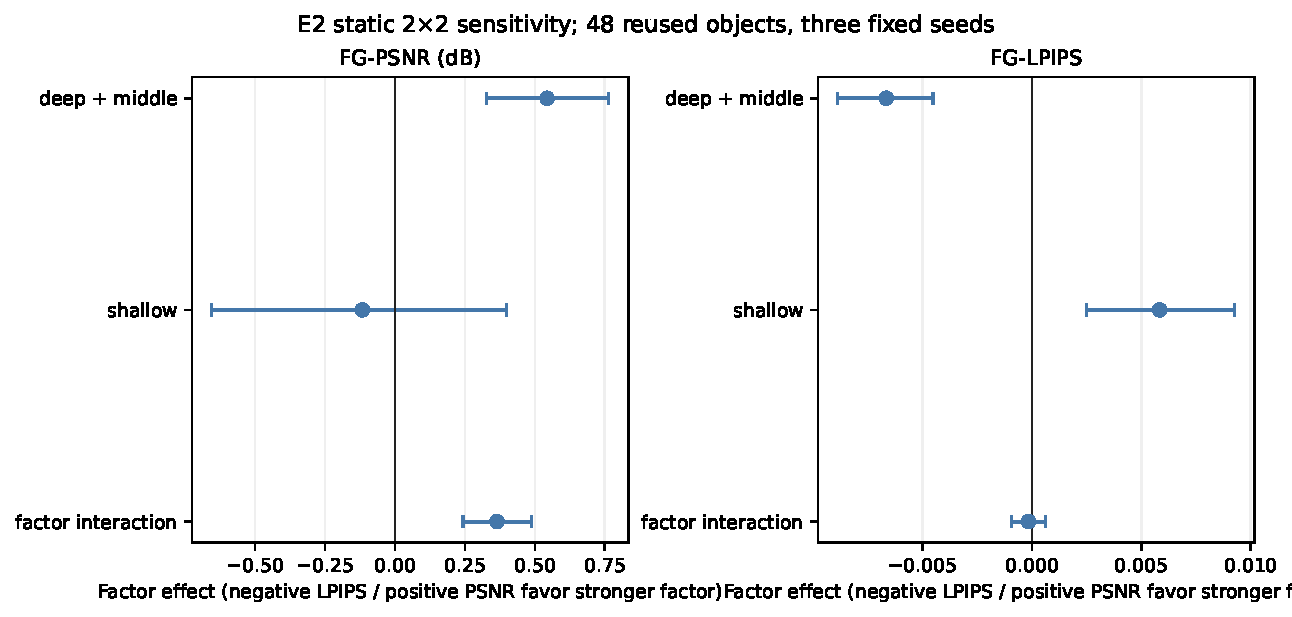
\includegraphics[width=0.94\linewidth]{e2_static_factors.pdf}
\caption{Object-bootstrap estimates for the three E2 factorial effects. The deep+middle-by-shallow interaction is endpoint-specific.}
\end{figure}

The primary interaction is not a temporal interaction. The formal design and row-accounting audit verify 576 logical rows (480 newly generated and 96 verified seed-42 reuses), 216,000 residual-trace entries, and 1,152 prediction/trace file hashes. The seed-42 F01 label requested 1.25 for shallow but the native cap applied 0.80; its predictions and effective trace match the 0.80 request. This request-field discrepancy is preserved in the alias erratum.

\section{S4. Bounded layer-by-window map and dose limits}

A3b covers 15 layer-by-window interventions relative to the all-low reference. The cluster-Wald and GEE tests detect response heterogeneity (FG-LPIPS interaction RMSE 0.000342; FG-PSNR 0.0205 dB). The dose calibration target was missed: deep and middle were approximately 20\% below target, while shallow was 98.98\% above target. The adjusted three-layer dose model retains 0/2,250 rows in common support. Therefore the response-surface test is not interpreted as a dose-independent mechanism. A2 is discovery evidence and is not used as an independent confirmatory replication.

\section{S5. GLB-native evaluation and visual audit}

The stored GLBs were rendered with their embedded glTF base-color sampler and frozen camera protocol. Source GLB hashes (160) and rendered image hashes (1,760) passed. Each object mean pools 11 unseen views. No texture was rebaked. The endpoint is unlit base-color and does not establish full-PBR appearance. Four objects without UVs were excluded before baking, so strict N=24 3D coverage is unsupported. The old seam analyzer is not treated as valid evidence for the exported mapping; no seam claim is made.

The 24-object 2D visual cohort was fixed using ground-truth-only strata before method outcomes. Each panel compares the same six target views for ground truth and seven generated conditions, including no adapter and fixed-scale controls. The panels are a completeness-oriented visual record; they are not a blinded human rating. Manual inspection recorded material/color mismatch in 18/24 objects and fine-detail loss in 21/24. Individual source-object attribution appears in S10.

\begin{figure}[p]
\centering
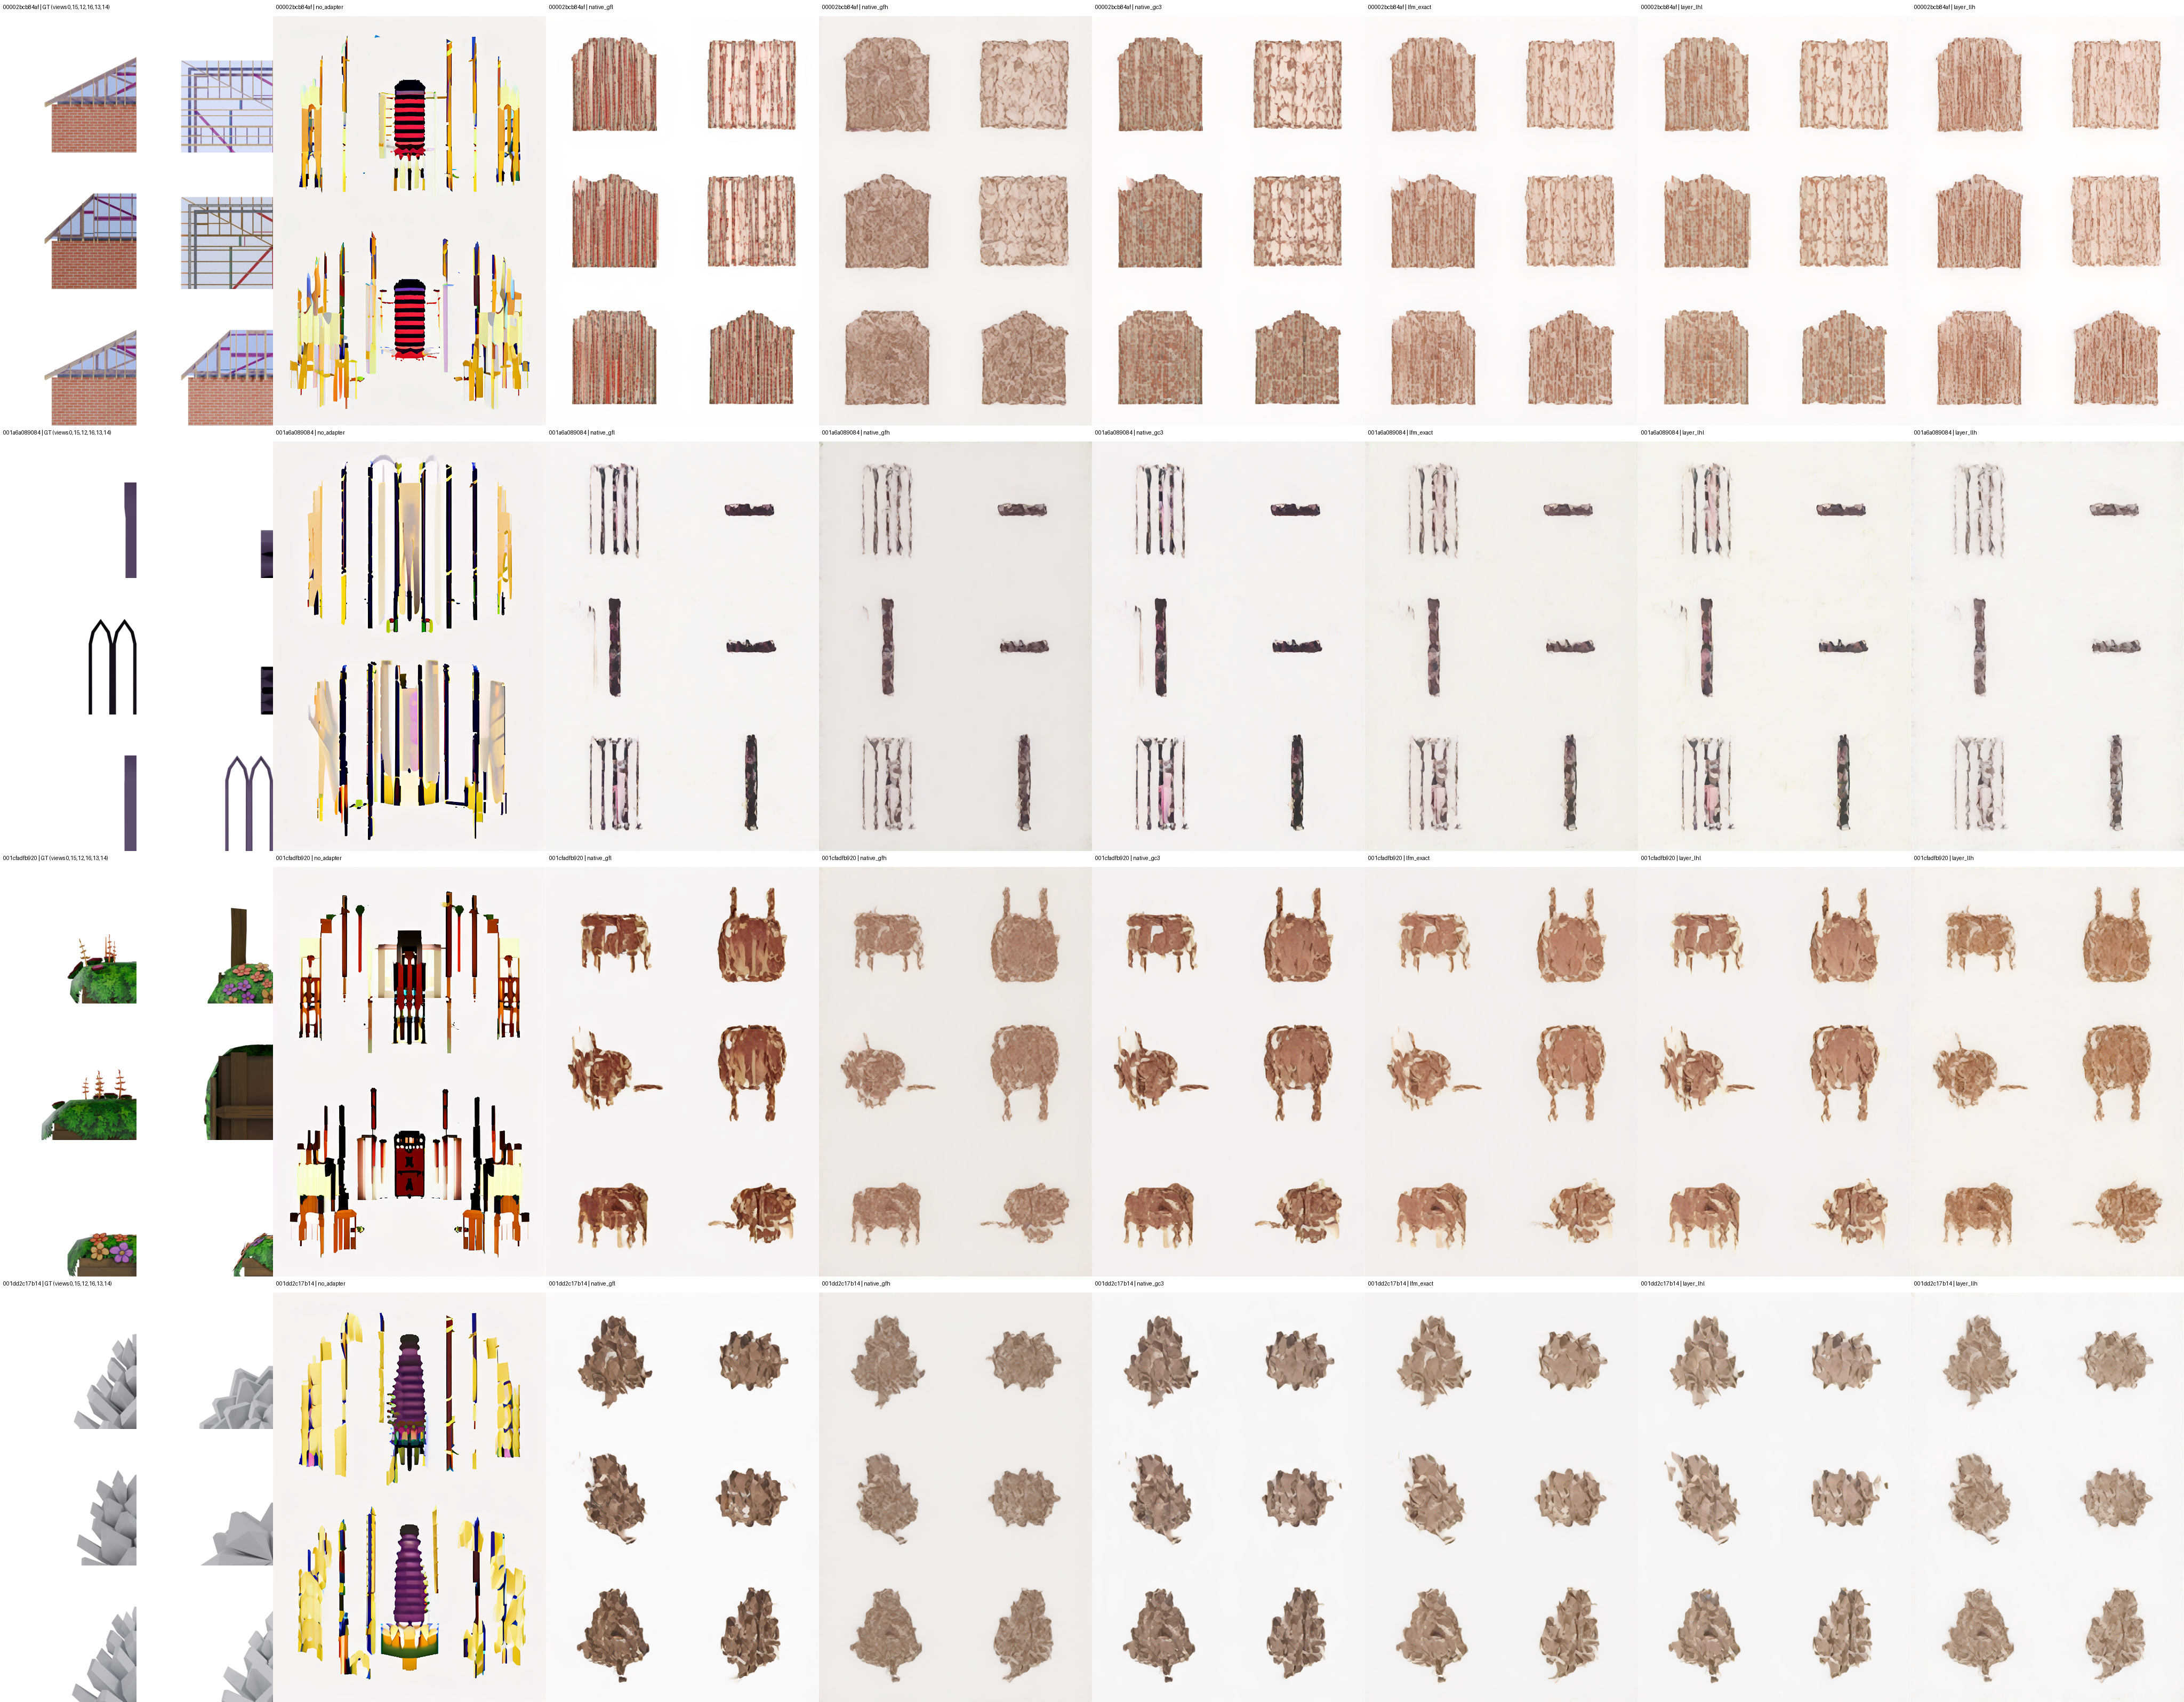
\includegraphics[width=\textwidth,height=0.82\textheight,keepaspectratio]{contact_sheet_parts/objects_01_04.jpg}
\caption{Preselected GT-stratified visual cohort, objects 1--4 of 24. Each row contains the fixed target views and same-draw outputs for the unmodified pipeline, native fixed-low and fixed-high baselines, GC3, LFM-exact, LHL, and LLH. Descriptive only; columns do not imply a ranking and do not evaluate the baked GLB endpoint.}
\end{figure}

\begin{figure}[p]
\centering
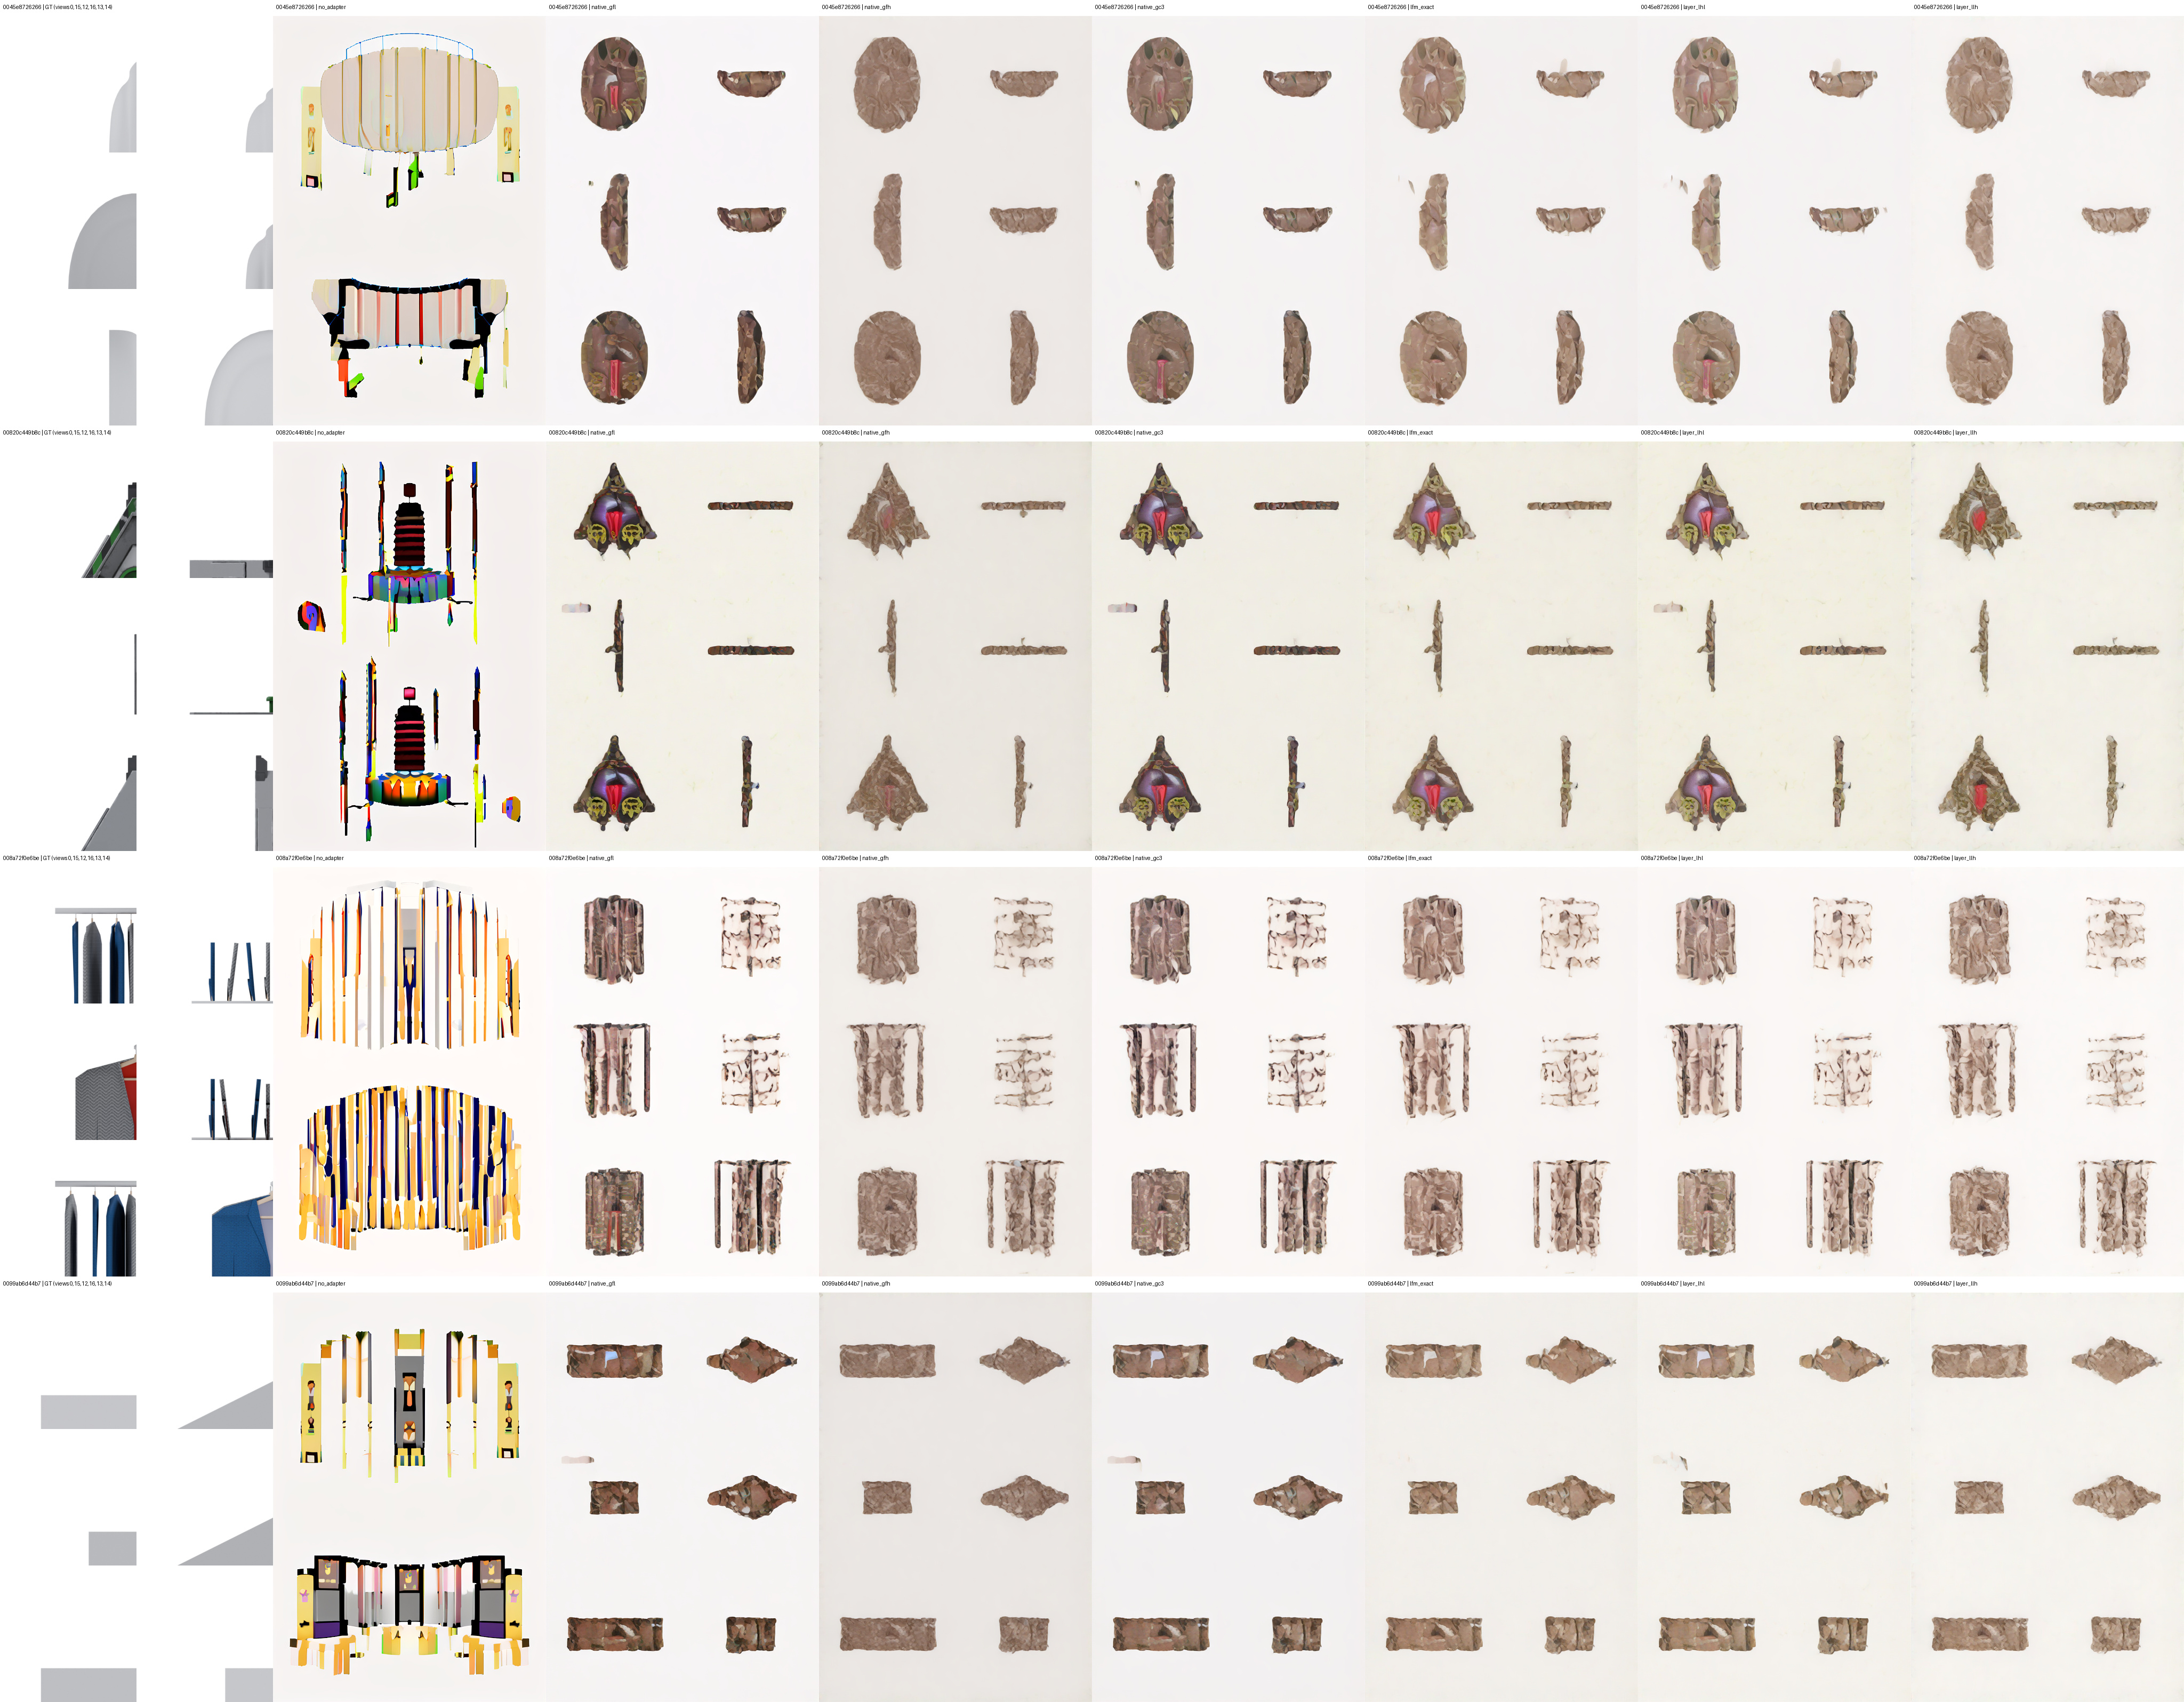
\includegraphics[width=\textwidth,height=0.82\textheight,keepaspectratio]{contact_sheet_parts/objects_05_08.jpg}
\caption{Preselected GT-stratified visual cohort, objects 5--8 of 24. Conditions and fixed target views match Fig. S1.}
\end{figure}

\begin{figure}[p]
\centering
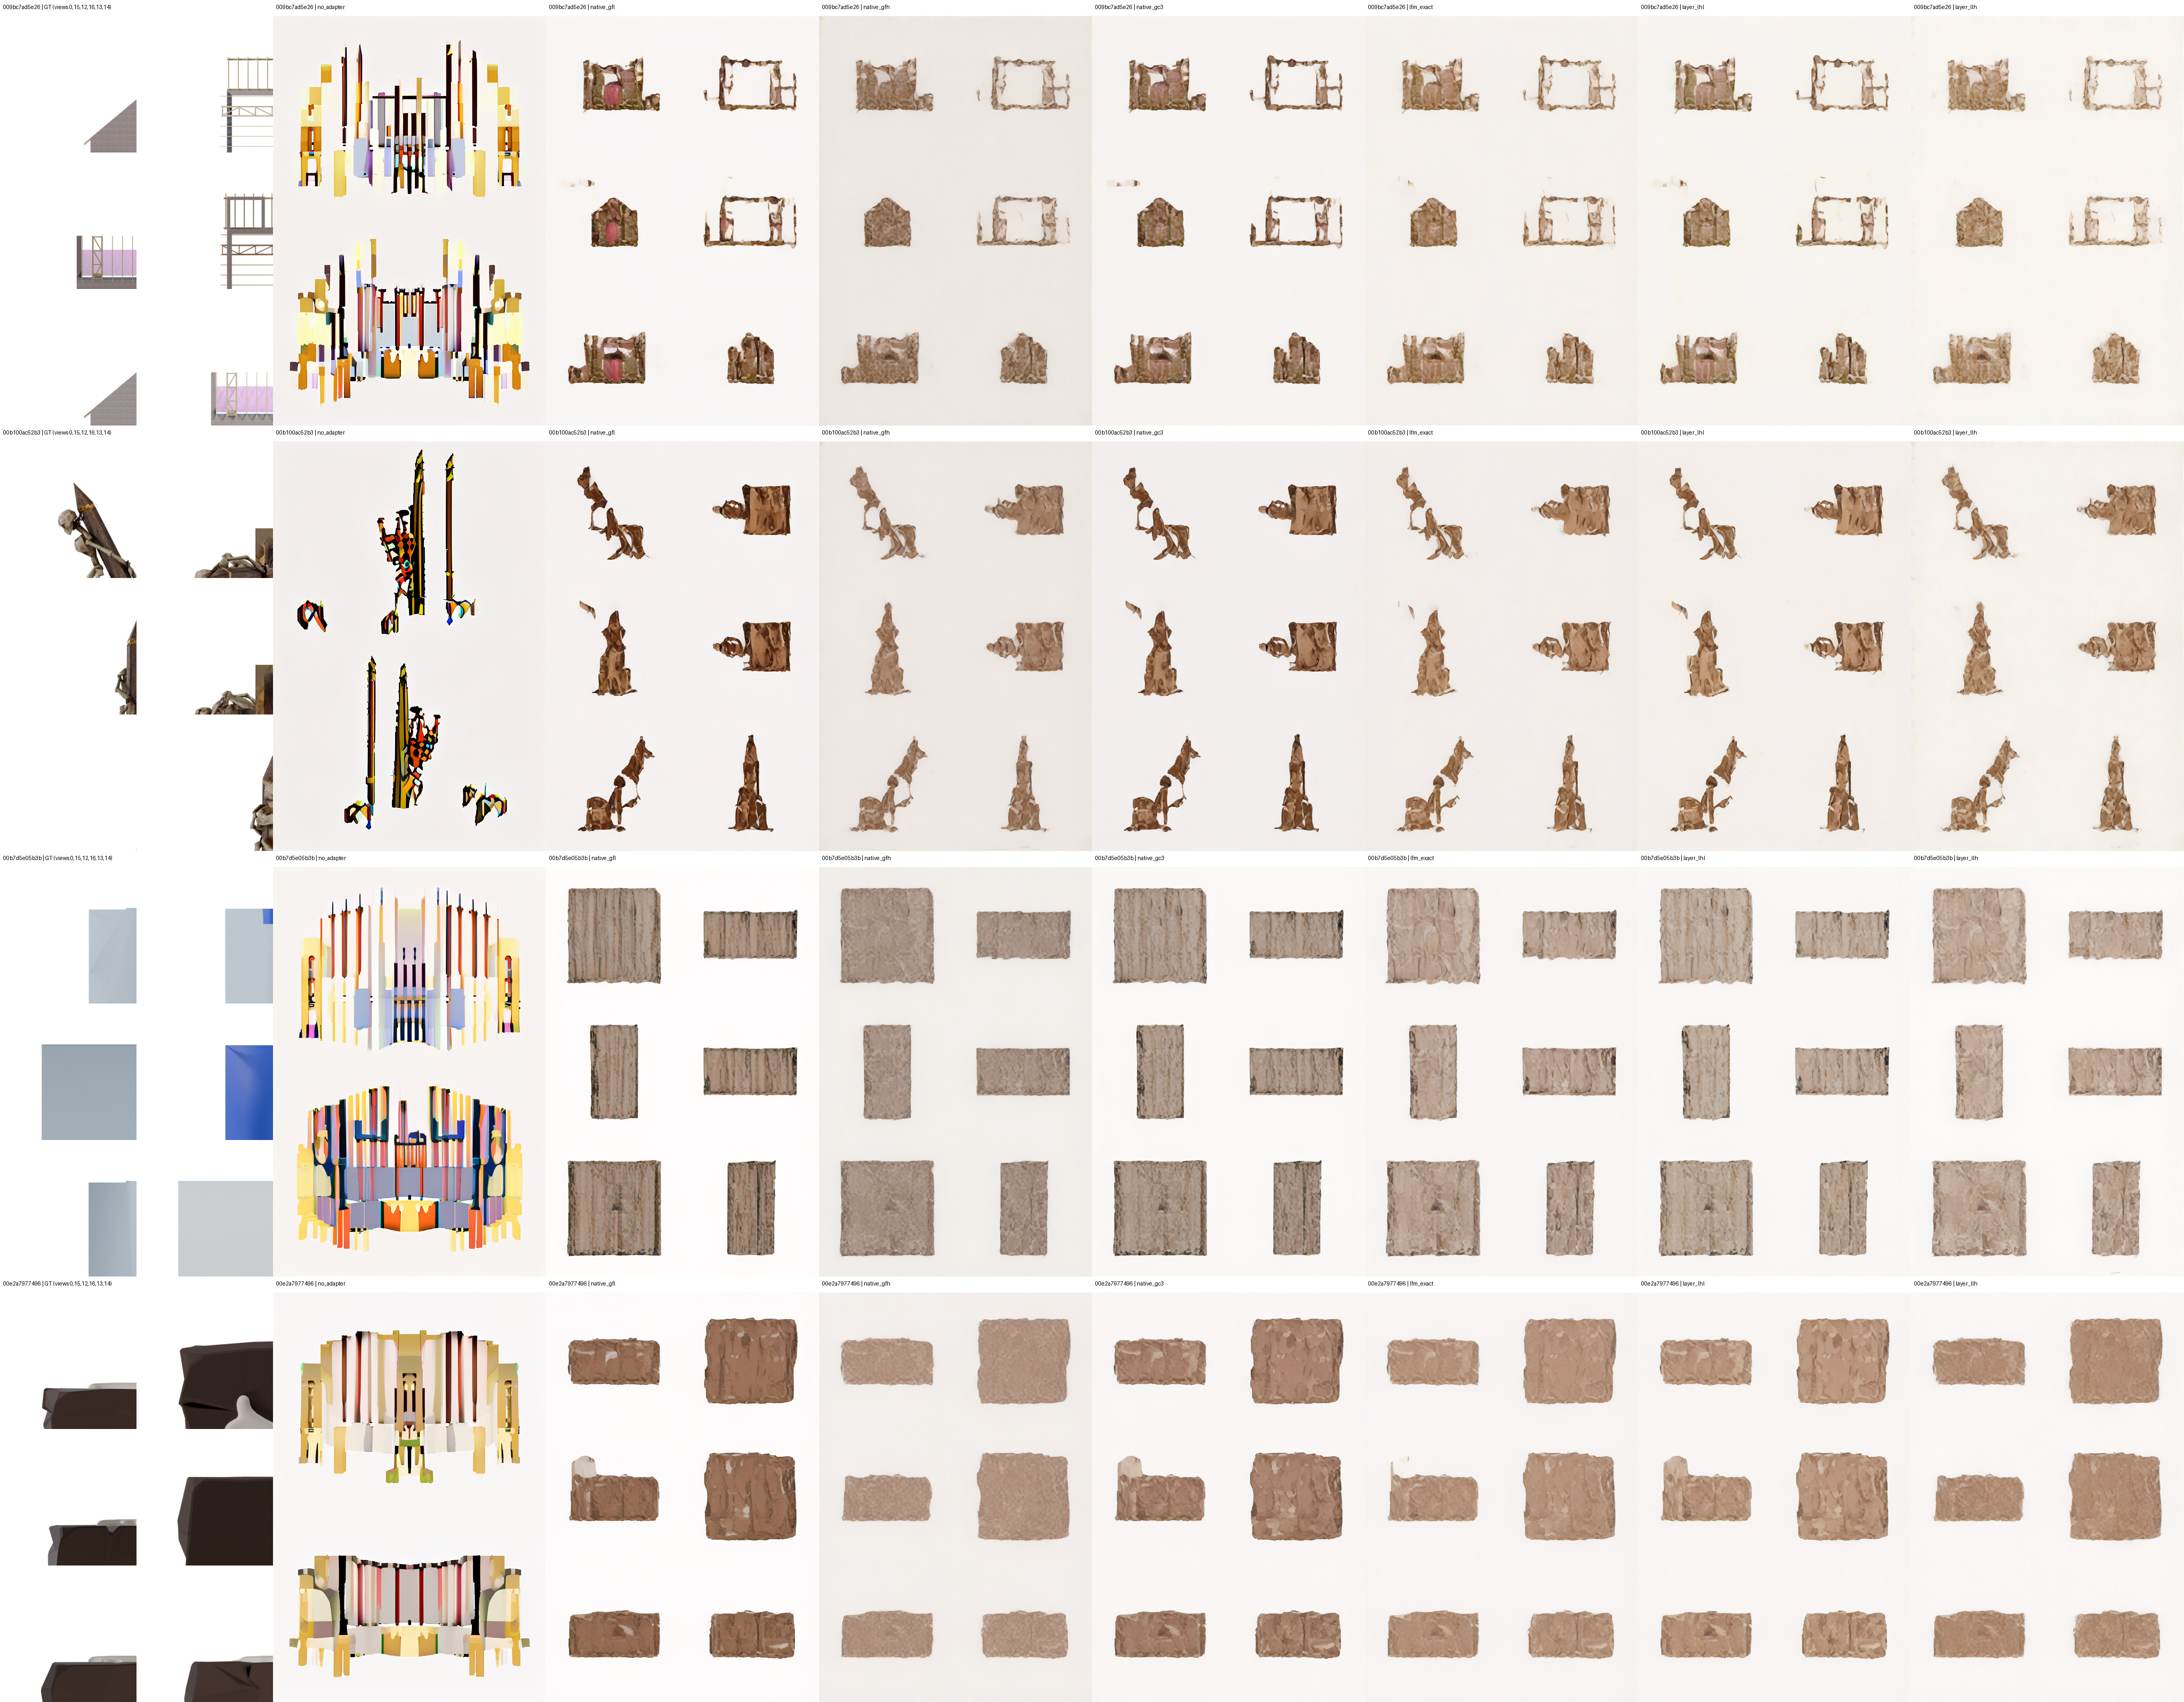
\includegraphics[width=\textwidth,height=0.82\textheight,keepaspectratio]{contact_sheet_parts/objects_09_12.jpg}
\caption{Preselected GT-stratified visual cohort, objects 9--12 of 24. Conditions and fixed target views match Fig. S1.}
\end{figure}

\begin{figure}[p]
\centering
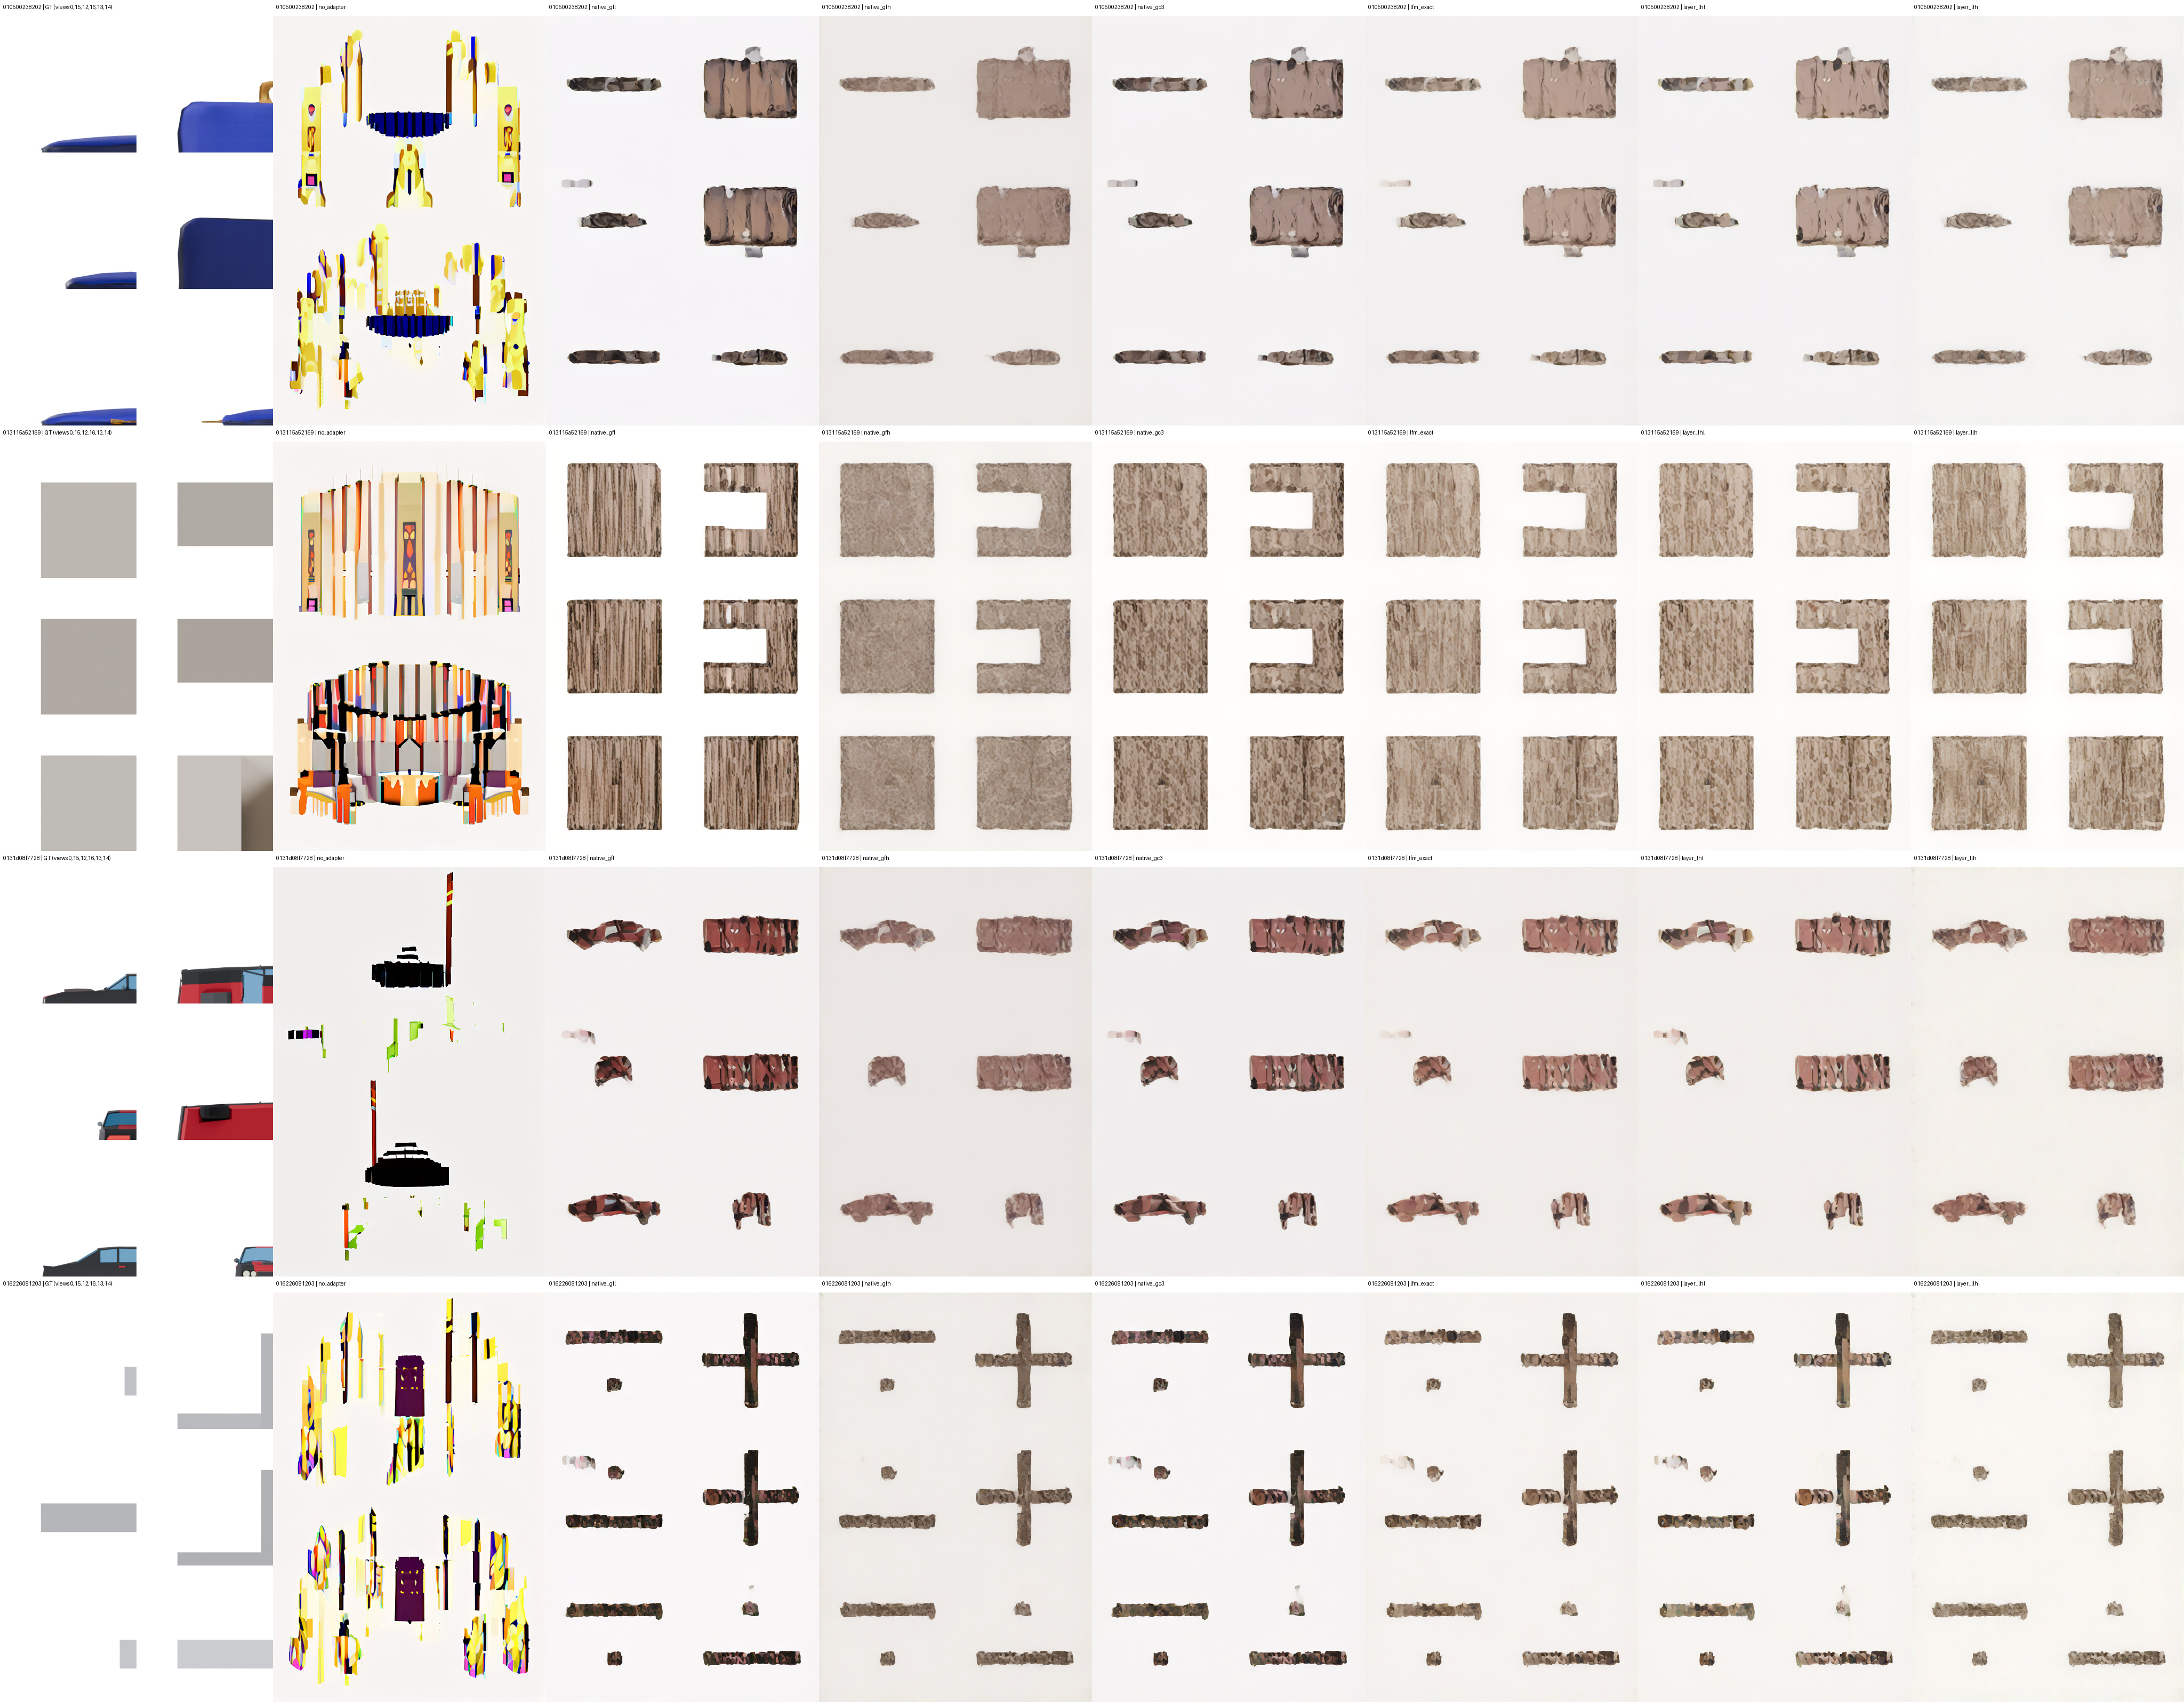
\includegraphics[width=\textwidth,height=0.82\textheight,keepaspectratio]{contact_sheet_parts/objects_13_16.jpg}
\caption{Preselected GT-stratified visual cohort, objects 13--16 of 24. Conditions and fixed target views match Fig. S1.}
\end{figure}

\begin{figure}[p]
\centering
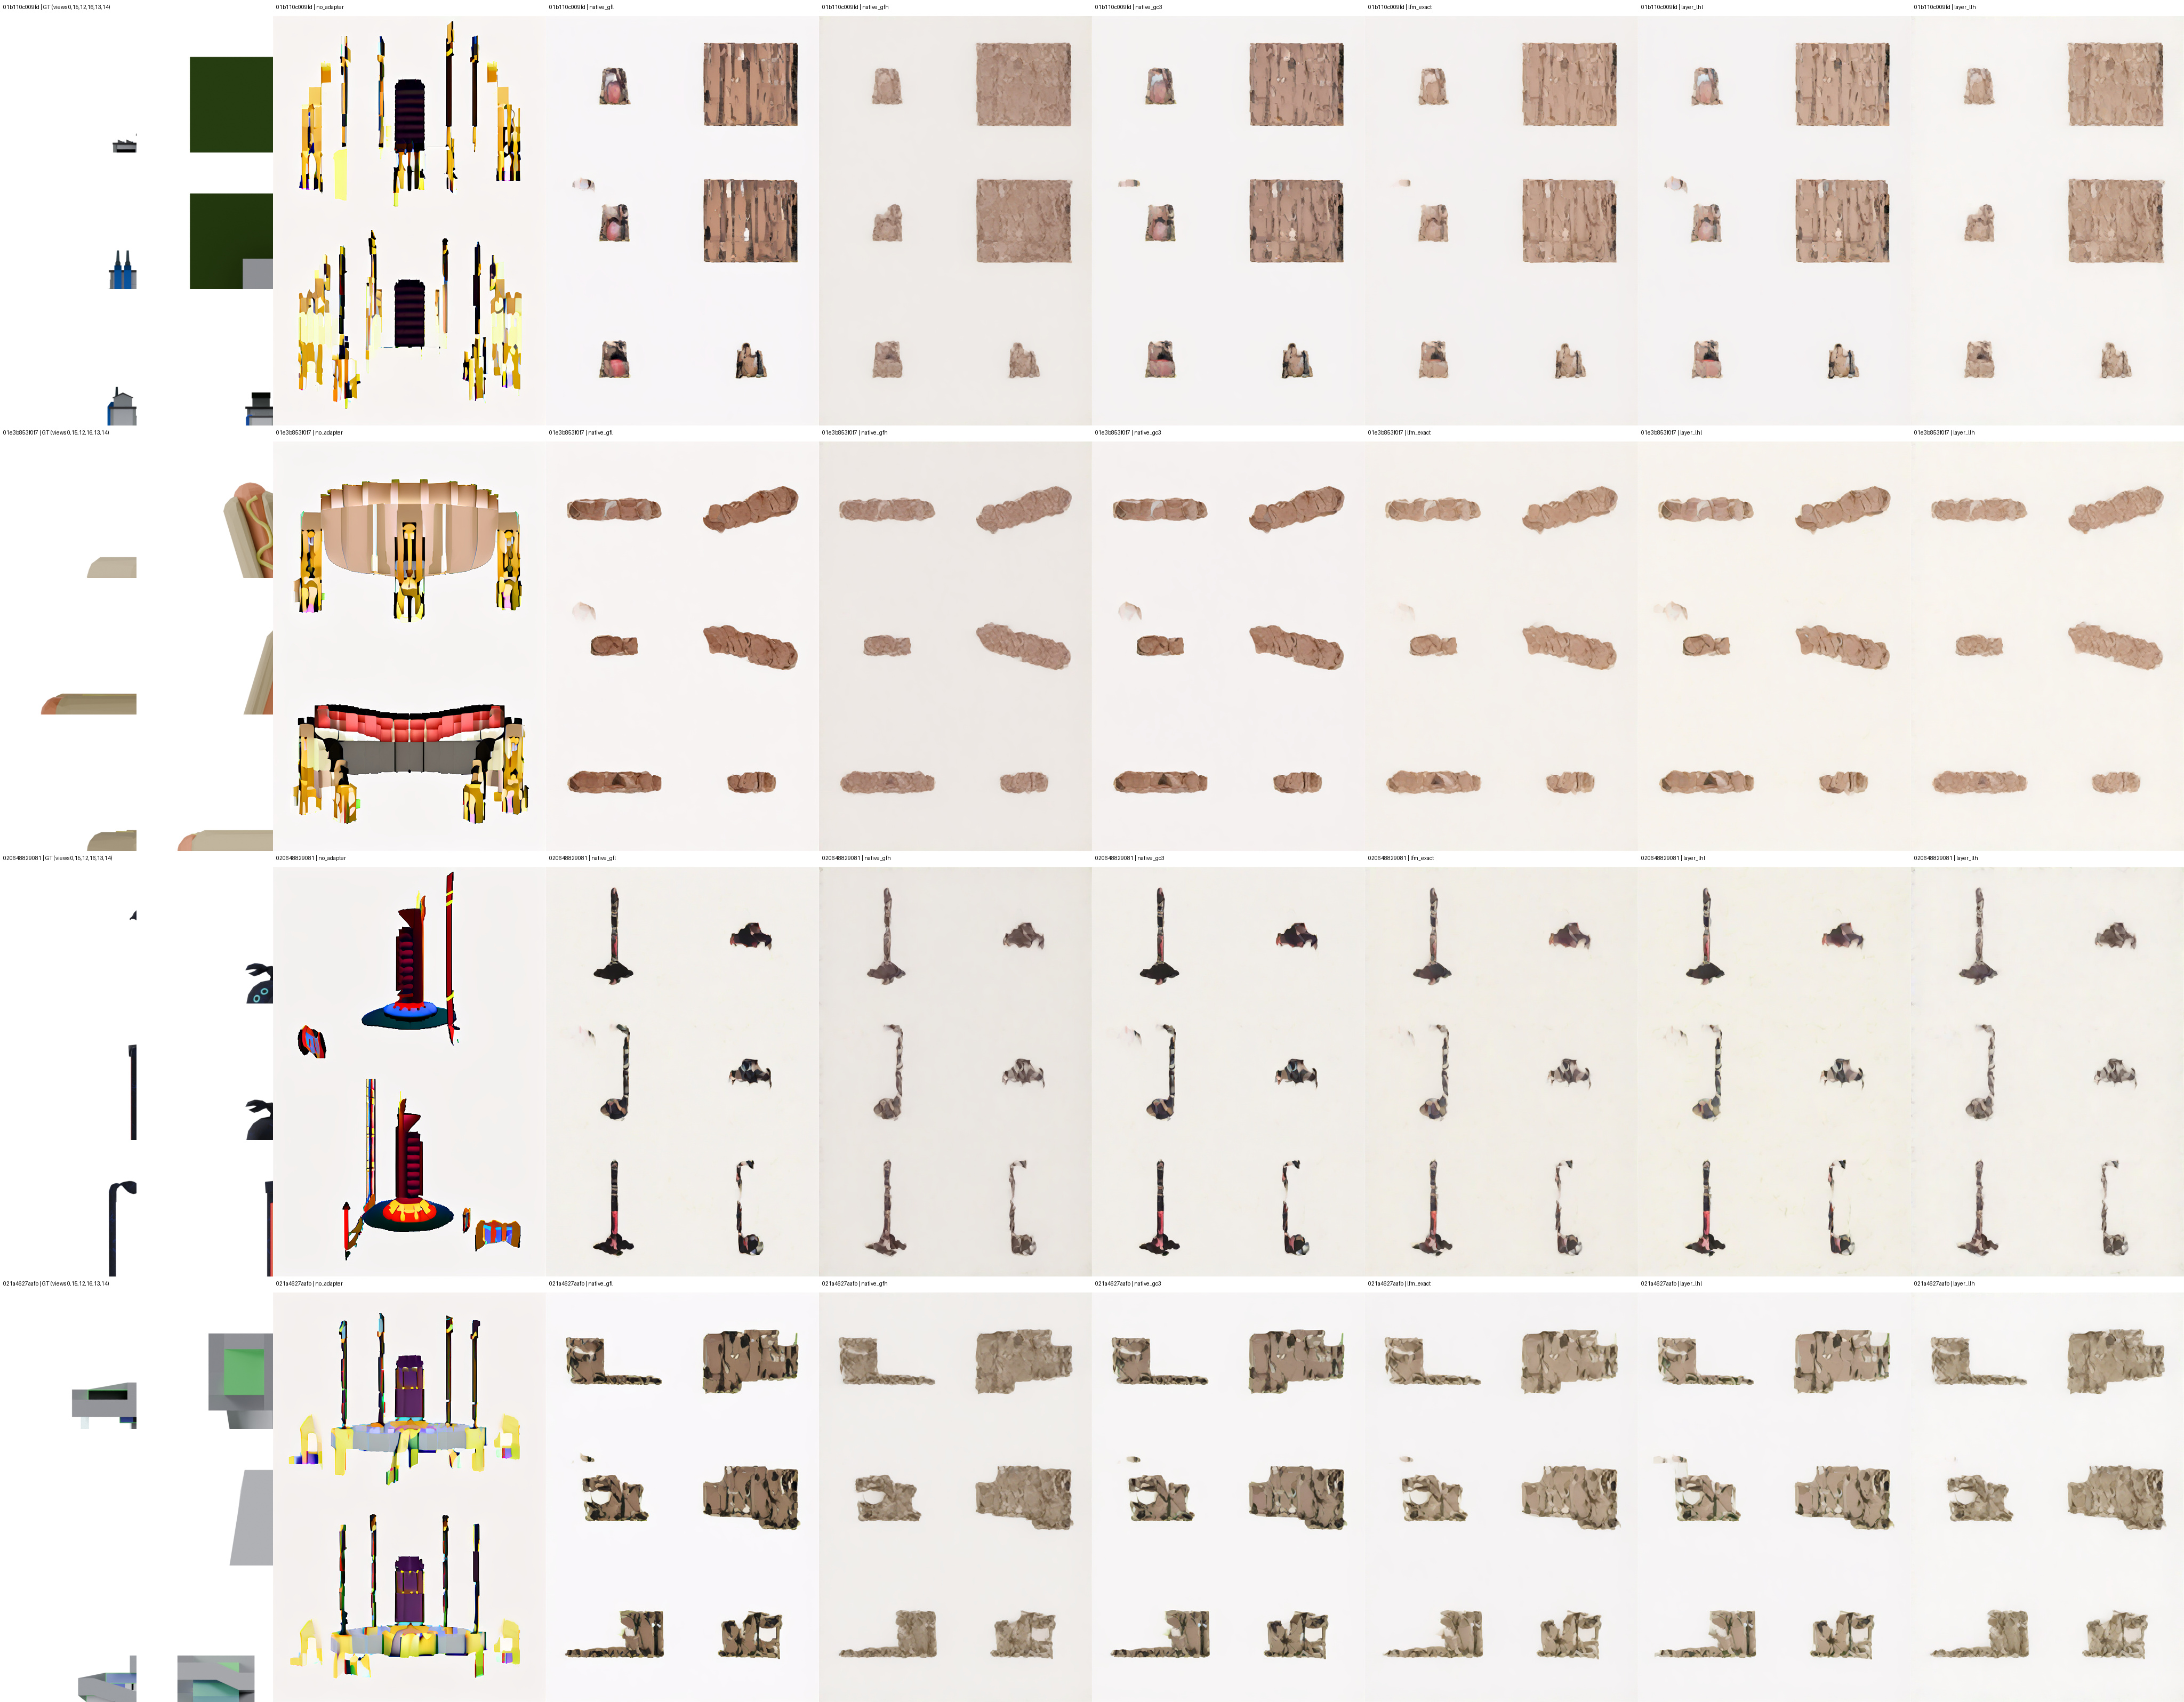
\includegraphics[width=\textwidth,height=0.82\textheight,keepaspectratio]{contact_sheet_parts/objects_17_20.jpg}
\caption{Preselected GT-stratified visual cohort, objects 17--20 of 24. Conditions and fixed target views match Fig. S1.}
\end{figure}

\begin{figure}[p]
\centering
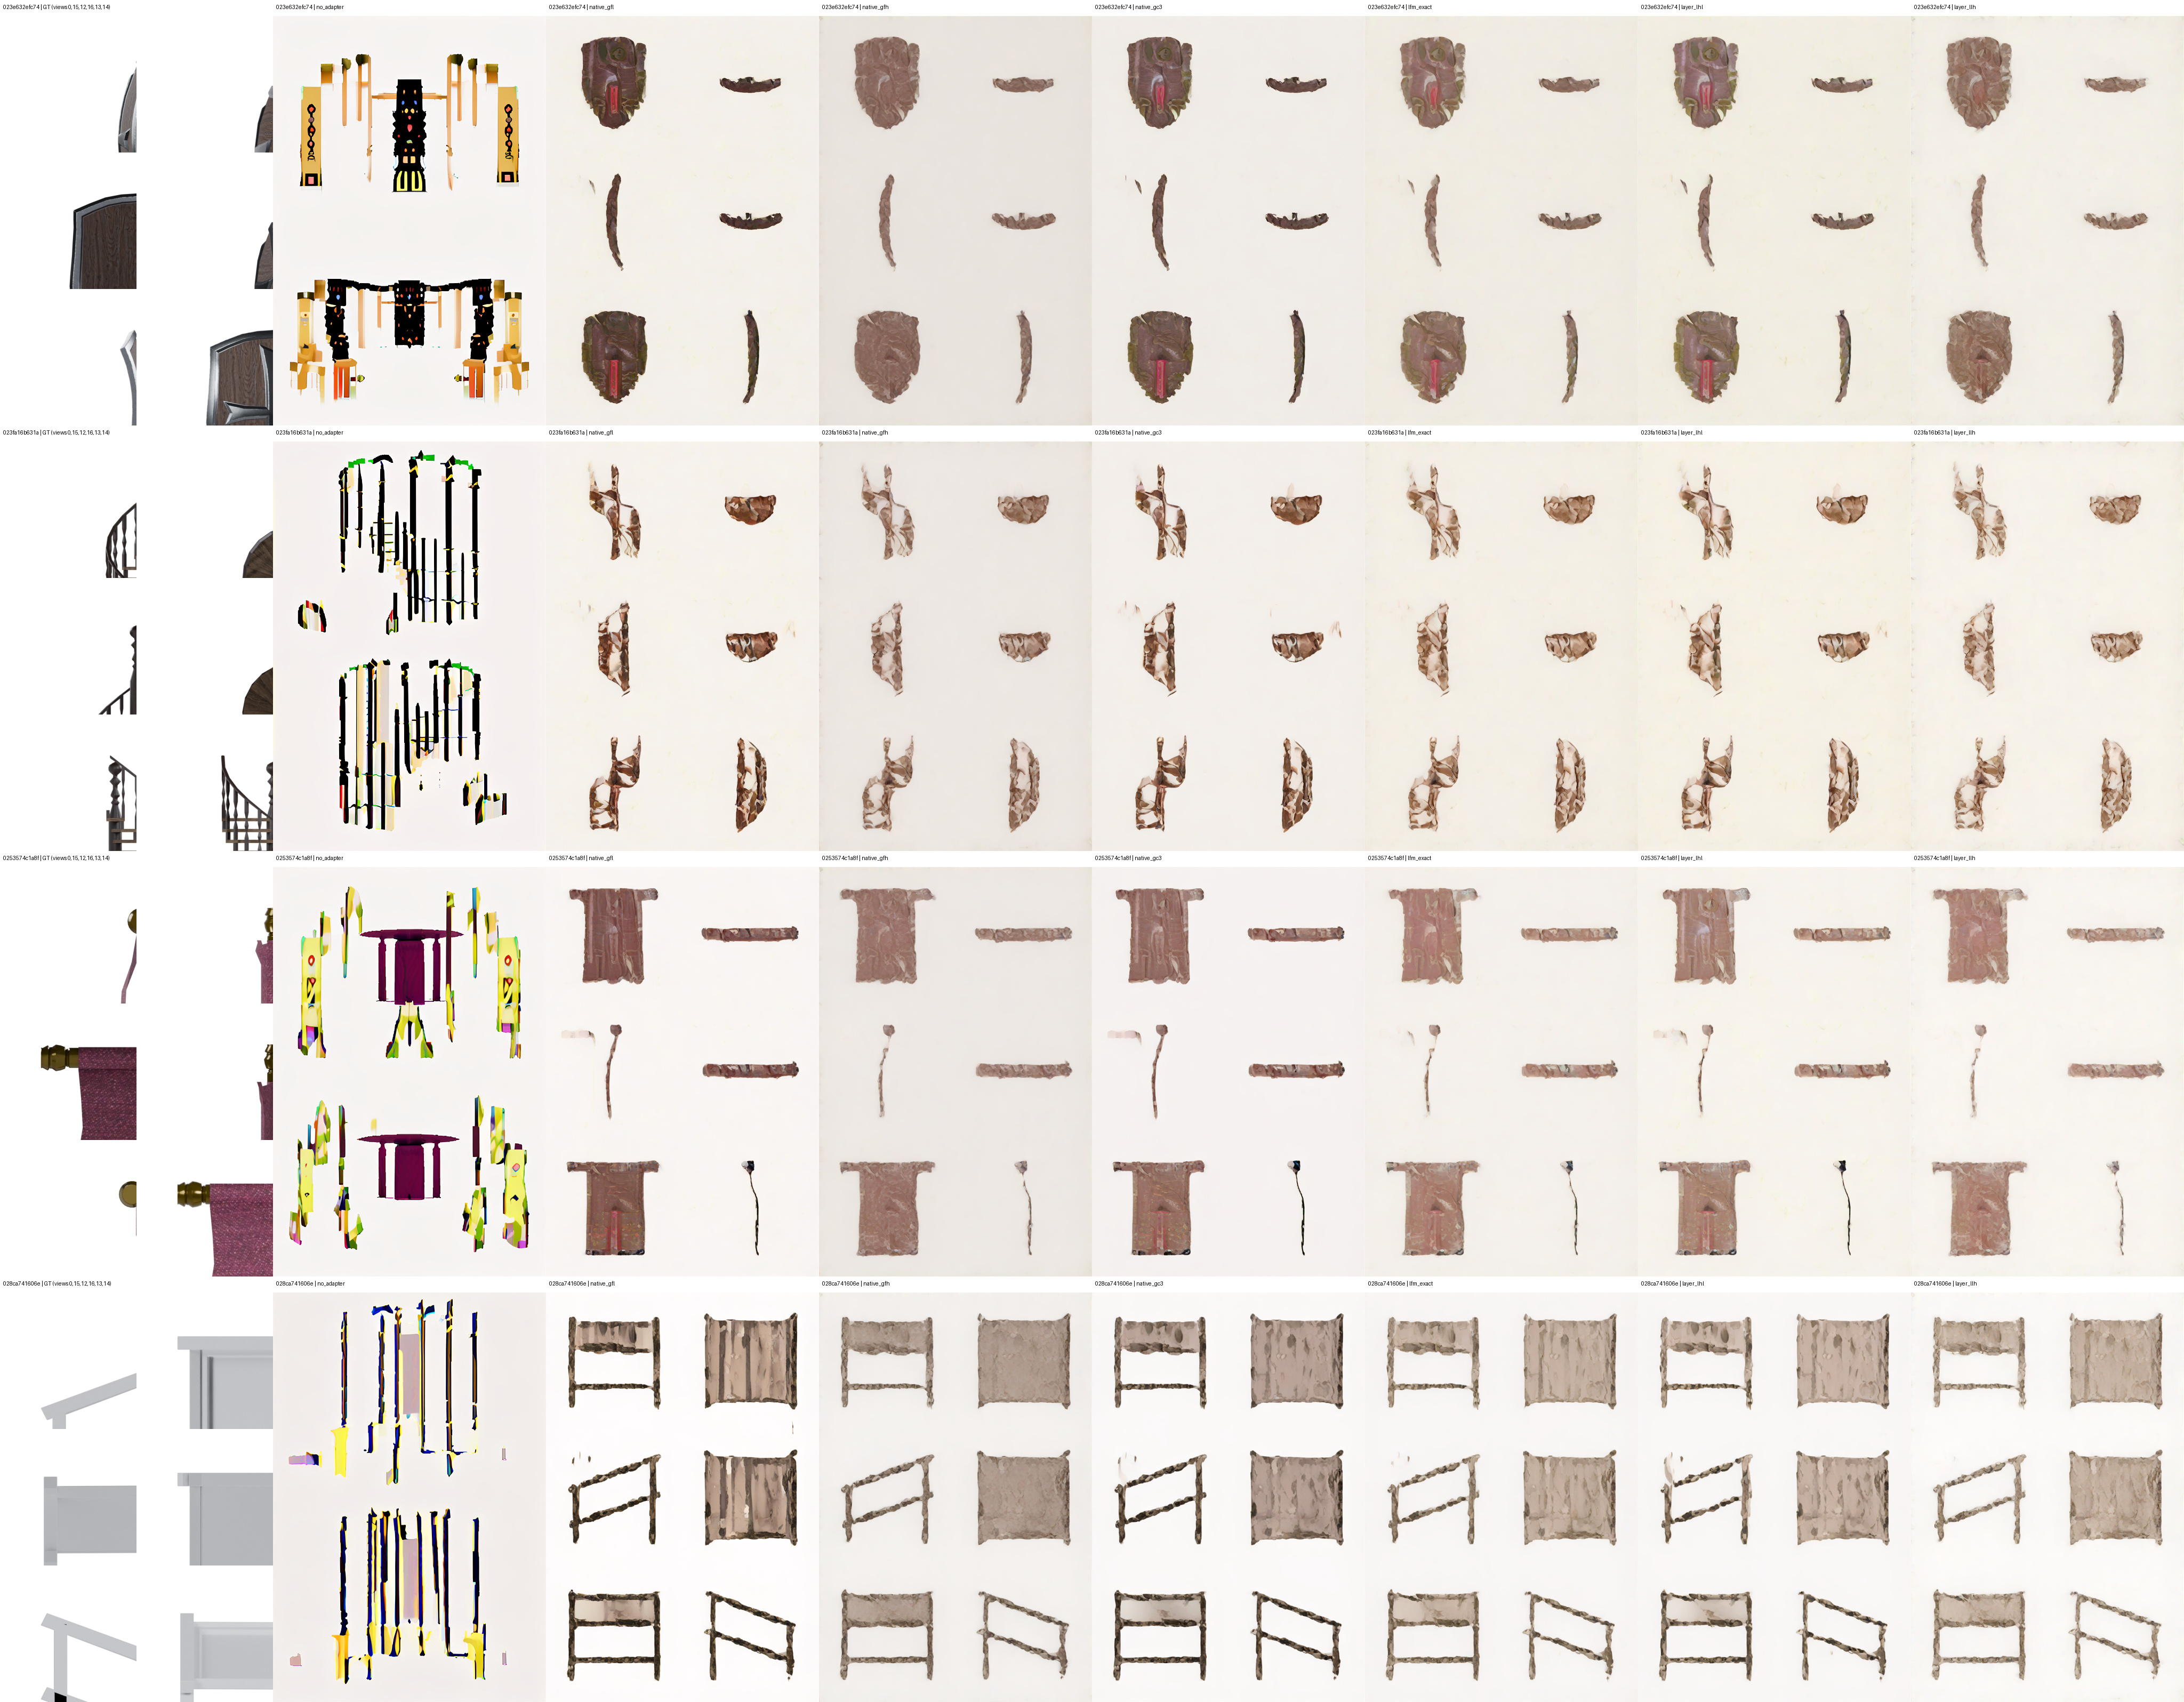
\includegraphics[width=\textwidth,height=0.82\textheight,keepaspectratio]{contact_sheet_parts/objects_21_24.jpg}
\caption{Preselected GT-stratified visual cohort, objects 21--24 of 24. Conditions and fixed target views match Fig. S1.}
\end{figure}

\begin{figure*}[p]
\centering
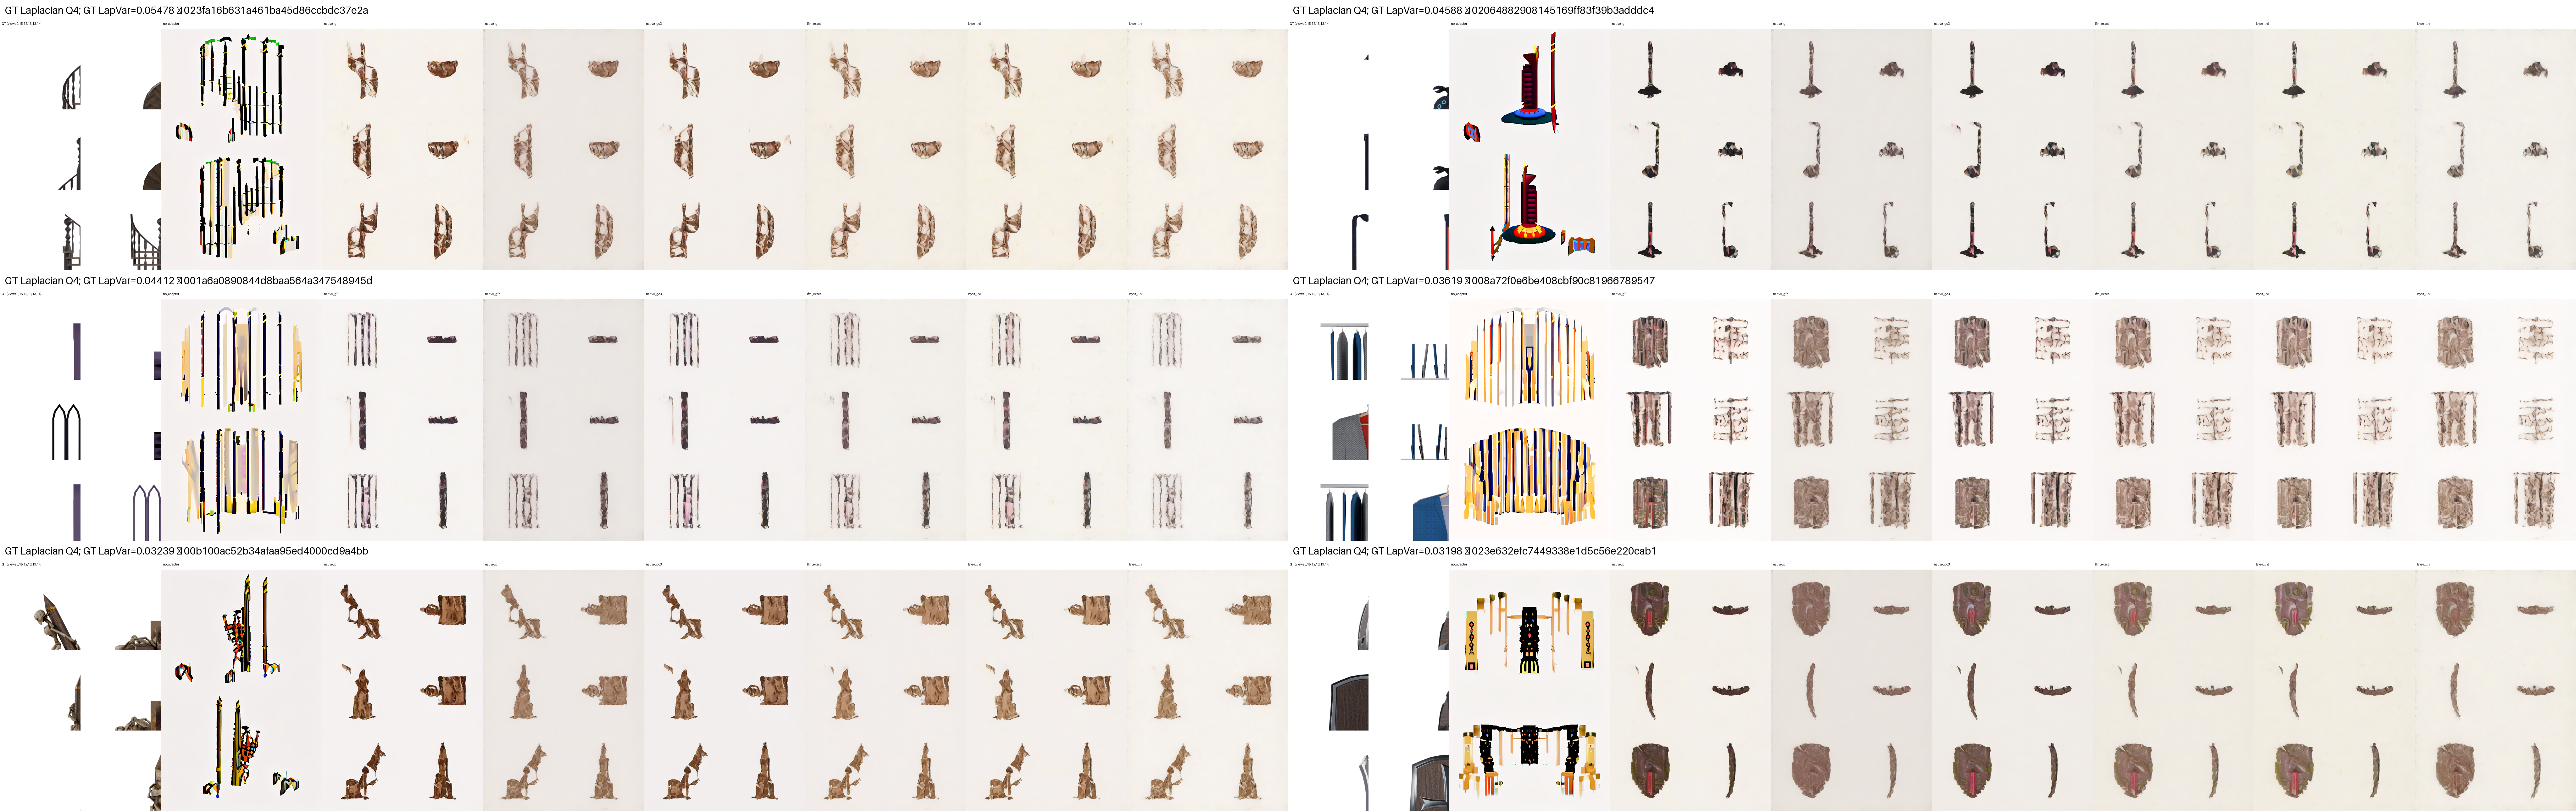
\includegraphics[width=\textwidth]{texture_rich_failure_sheet.png}
\caption{Six highest ground-truth Laplacian-variance objects within the same fixed 24-object cohort, shown across the recorded conditions. This outcome-independent subset is descriptive and does not estimate a population failure rate.}
\end{figure*}

Metric-ranked strongest-win, median-effect, and strongest-loss panels are available in \texttt{manuscript/figures/}; they are selected illustrations from the 24-object visual cohort, not independent evidence. Their rank rule and object IDs are in the copied visual-evidence report.

\section{S6. Retrospective C3 paired re-evaluations}

All estimates in S6 are retrospective object-paired supplements. The strict-276 GC3--GFL and GC3--GFH pairs were not registered primary Core-7 contrasts; legacy GFL/GC3 input-tensor hashes and common-runner identity are incomplete. FRESH\_CONFIRM\_B is a disjoint 150-object cohort, but it was already unblinded and the native-GC3--native-GFL B3 pair was not registered. The B pair therefore has an independent object set but is post hoc, not an independent prospective or registered confirmation. Every interval below is an unadjusted, nominal percentile object-bootstrap 95\% CI; favorable-object direction is high for PSNR, SSIM, and Edge-SSIM, and low for LPIPS. Exact object-level deltas and analysis scripts are included in \texttt{data/derived/} and \texttt{scripts/}.

\begin{table}[p]
\centering\scriptsize
\caption{Strict-276 retrospective GC3 paired differences. Delta is GC3 minus the comparator.}
\label{tab:strict276-c3}
\begin{tabular}{p{1.4cm}p{4.4cm}p{1.3cm}p{4.4cm}p{1.3cm}}
\toprule
Endpoint & GC3 $-$ GFL mean [95\% CI] & Favorable & GC3 $-$ GFH mean [95\% CI] & Favorable \\
\midrule
FG-PSNR (dB) & +1.208 [1.117, 1.295] & 259/276 & -1.214 [-1.314, -1.115] & 25/276 \\
FG-SSIM & +0.03086 [0.02832, 0.03335] & 261/276 & -0.04878 [-0.05154, -0.04590] & 7/276 \\
FG-LPIPS & -0.01003 [-0.01093, -0.00912] & 248/276 & +0.01396 [0.01298, 0.01491] & 13/276 \\
Full-PSNR (dB) & +0.7389 [0.6476, 0.8275] & 226/276 & +0.7252 [0.6471, 0.8065] & 240/276 \\
Full-SSIM & +0.007184 [0.006571, 0.007781] & 253/276 & +0.001229 [0.000570, 0.001886] & 187/276 \\
Full-LPIPS & -0.007819 [-0.008780, -0.006851] & 228/276 & +0.006176 [0.004968, 0.007341] & 76/276 \\
Edge-SSIM & +0.007760 [0.006773, 0.008746] & 233/276 & -0.02601 [-0.02804, -0.02399] & 18/276 \\
\bottomrule
\end{tabular}
\end{table}

\begin{table}[p]
\centering\scriptsize
\caption{FRESH\_CONFIRM\_B post-hoc native-GC3 minus native-GFL differences. Holm $p$ values are an exploratory sensitivity across seven endpoints and do not make the contrast registered.}
\label{tab:freshb-c3}
\begin{tabular}{p{1.8cm}p{5.2cm}p{1.4cm}p{1.4cm}}
\toprule
Endpoint & Mean difference [nominal 95\% CI] & Favorable objects & Post-hoc Holm $p$ \\
\midrule
FG-PSNR (dB) & +0.502 [0.342, 0.663] & 100/150 & 0.0007 \\
FG-SSIM & +0.02380 [0.01911, 0.02901] & 123/150 & 0.0007 \\
FG-LPIPS & -0.00513 [-0.00655, -0.00369] & 107/150 & 0.0007 \\
Full-PSNR (dB) & +0.225 [0.095, 0.358] & 82/150 & 0.0007 \\
Full-SSIM & +0.005934 [0.004797, 0.007107] & 130/150 & 0.0007 \\
Full-LPIPS & -0.004548 [-0.006102, -0.003009] & 109/150 & 0.0007 \\
Edge-SSIM & +0.005034 [0.003348, 0.006753] & 105/150 & 0.0007 \\
\bottomrule
\end{tabular}
\end{table}

On strict-276, all seven GC3--GFL endpoint directions favor GC3, whereas only full-image PSNR and SSIM favor GC3 over fixed-high; foreground and edge metrics favor fixed-high. On the disjoint B objects, all seven mean directions favor GC3 over GFL, but this post-hoc analysis cannot erase the earlier exposure or be treated as a fresh registered replication. The historic pooled +0.96 dB is not carried forward as an independently confirmed effect.

\section{S7. Cross-interface results}

The MV-Adapter experiment evaluates 98 objects from 99 planned across a bounded one-window additive-residual intervention. No global interaction survives the exploratory four-metric correction; isolated late shallow LPIPS changes are small and do not establish a general null or a transfer law.

MVDiffusion is a separate 75-object result on the unchanged SD2-depth compatibility deployment base. Its schedule interpolates serial correspondence-aware CPBlock outputs, not an independent geometry-residual branch. For layer-LLH versus global fixed-low, paired means trade structural/color endpoints against GT-relative texture error: PSNR is -0.454 dB, FG-SSIM -0.0194, Edge-SSIM -0.0059, while CIEDE2000 is -1.373; FG-LPIPS is not separated. This is a boundary for that interface and intervention, not a matched causal architecture comparison. Absolute scores are never pooled across these cohorts.

\section{S8. Human preference and scope}

No participant responses were collected for the current LLH comparisons. The frozen LLH study uses 40 fixed slots, 24 paired judgments per participant, eight endpoints, and at least 36 valid completions; its current response count is zero. The prior 01549 preference study compared different scale profiles and is not transferred to LLH, GLB unseen views, or material fidelity in this revision. The manuscript therefore makes no human-preference claim for current profiles. The response template and the frozen analysis/validation rules are included under \texttt{guides/} and \texttt{evidence/protocols/}.

\section{S9. Provenance and supersession}

The first authority for claim wording is \texttt{evidence/audits/next\_stage\_20261006/NARRATIVE\_DECISION\_MAP.md} together with the hash-validated claim-authority ledger. The GLB-native report supersedes the older CPU-renderer or seam summaries for stored exported GLBs. Fresh B is a disjoint object cohort but its lock chronology is retrospective. E1/E2 are fixed-subset sensitivity analyses. The strict-276 C3 contrast is retrospective. Full generated image and residual-trace outputs are omitted from this GitHub evidence copy because of size and redistribution constraints; their source hashes and original local paths remain indexed in the original audit manifests. Do not treat omitted payload hashes as a substitute for access to the payloads when a clean-clone reproduction is required.

\section{S10. Per-object visual asset attribution}

The 24-object visual cohort uses Objaverse 1.0 assets. The table maps each panel to its source UID and creator, and links the Sketchfab model page and Creative Commons license. Current API metadata corroborates 22/24 license records. For panel 02 the current API license field is empty; for panel 05 the model endpoint returns 404. Both retain the Objaverse snapshot \texttt{by} slug and are marked with $\dagger$. The stored description for panel 02 also refers to personal-project use, so its redistribution terms need author-level confirmation before the final public release. The ShareAlike asset in panel 06 is separately identified; any redistribution of an adaptation must honor its terms. No source meshes are included in this package.

\small
\begin{longtable}{r p{3.4cm} p{4.3cm} p{2.7cm} p{2.0cm}}
\caption{Source and license attribution for the fixed visual panel.}\\
\toprule
Panel & Source UID / model page & Creator & License & API record \\
\midrule
\endfirsthead
\toprule
Panel & Source UID / model page & Creator & License & API record \\
\midrule
\endhead
\bottomrule
\endfoot
00 & \href{https://sketchfab.com/3d-models/00002bcb84af4a4781174e62619f14e2}{Sketchfab model page} & \href{https://sketchfab.com/mstam}{mstam} & \href{https://creativecommons.org/licenses/by/4.0/}{CC BY 4.0} & live API \\
01 & \href{https://sketchfab.com/3d-models/001a6a0890844d8baa564a347548945d}{Sketchfab model page} & \href{https://sketchfab.com/UltraMelon}{UltraMelon} & \href{https://creativecommons.org/licenses/by/4.0/}{CC BY 4.0} & live API \\
02 & \href{https://sketchfab.com/3d-models/001cfadfb9204424bccc45501ce6b90e}{Sketchfab model page} & \href{https://sketchfab.com/johnguataquira}{johnguataquira} & \href{https://creativecommons.org/licenses/by/4.0/}{CC BY 4.0$^{\dagger}$} & snapshot only$^{\dagger}$ \\
03 & \href{https://sketchfab.com/3d-models/001dd2c17b1443aab500f61634bc3b89}{Sketchfab model page} & \href{https://sketchfab.com/ie-niels}{IronEqual} & \href{https://creativecommons.org/licenses/by/4.0/}{CC BY 4.0} & live API \\
04 & \href{https://sketchfab.com/3d-models/0045e87262664927a3298f2ed0f640c1}{Sketchfab model page} & \href{https://sketchfab.com/avroralepnina}{AVRORA Group} & \href{https://creativecommons.org/licenses/by/4.0/}{CC BY 4.0} & live API \\
05 & \href{https://sketchfab.com/3d-models/00820c449b8c4c84b3ae58d3d168ca7b}{Sketchfab model page} & \href{https://sketchfab.com/flomezsupercool}{Flomezsupercool3 / coolpurpleguy} & \href{https://creativecommons.org/licenses/by/4.0/}{CC BY 4.0$^{\dagger}$} & snapshot only$^{\dagger}$ \\
06 & \href{https://sketchfab.com/3d-models/008a72f0e6be408cbf90c81966789547}{Sketchfab model page} & \href{https://sketchfab.com/1-3D.com}{1-3D.com} & \href{https://creativecommons.org/licenses/by-sa/4.0/}{CC BY-SA 4.0} & live API \\
07 & \href{https://sketchfab.com/3d-models/0099ab6d44b742b0b62a40a7c70c29b1}{Sketchfab model page} & \href{https://sketchfab.com/127469}{127469} & \href{https://creativecommons.org/licenses/by/4.0/}{CC BY 4.0} & live API \\
08 & \href{https://sketchfab.com/3d-models/009bc7ad5e26471198c8e5e41637fc60}{Sketchfab model page} & \href{https://sketchfab.com/pesek_martinice}{MARTINICE GROUP} & \href{https://creativecommons.org/licenses/by/4.0/}{CC BY 4.0} & live API \\
09 & \href{https://sketchfab.com/3d-models/00b100ac52b34afaa95ed4000cd9a4bb}{Sketchfab model page} & \href{https://sketchfab.com/DocStephen}{DocStephen} & \href{https://creativecommons.org/licenses/by/4.0/}{CC BY 4.0} & live API \\
10 & \href{https://sketchfab.com/3d-models/00b7d5e05b3b404c944cf3f7c92d15ba}{Sketchfab model page} & \href{https://sketchfab.com/jorgebaby160}{jorgebaby} & \href{https://creativecommons.org/licenses/by/4.0/}{CC BY 4.0} & live API \\
11 & \href{https://sketchfab.com/3d-models/00e2a79774964cb08f38c4406407300b}{Sketchfab model page} & \href{https://sketchfab.com/tsutomu.saito}{tsutomu.saito} & \href{https://creativecommons.org/licenses/by/4.0/}{CC BY 4.0} & live API \\
12 & \href{https://sketchfab.com/3d-models/0105002382024c2a8c12ee2a9b778187}{Sketchfab model page} & \href{https://sketchfab.com/astridgarod}{astridgarod} & \href{https://creativecommons.org/licenses/by/4.0/}{CC BY 4.0} & live API \\
13 & \href{https://sketchfab.com/3d-models/013115a5216943f5b56641864b6c28d2}{Sketchfab model page} & \href{https://sketchfab.com/gmedranotic}{GmedranoTIC} & \href{https://creativecommons.org/licenses/by/4.0/}{CC BY 4.0} & live API \\
14 & \href{https://sketchfab.com/3d-models/0131d08f77284aea9c62ad6de74edc0b}{Sketchfab model page} & \href{https://sketchfab.com/Wordofcurse}{Wordofcurse} & \href{https://creativecommons.org/licenses/by/4.0/}{CC BY 4.0} & live API \\
15 & \href{https://sketchfab.com/3d-models/0162260812034687a4d337161f632d09}{Sketchfab model page} & \href{https://sketchfab.com/szaboo}{szaboo} & \href{https://creativecommons.org/licenses/by/4.0/}{CC BY 4.0} & live API \\
16 & \href{https://sketchfab.com/3d-models/01b110c009fd4bb3a0e25adb093c09a2}{Sketchfab model page} & \href{https://sketchfab.com/sanchibbo}{SANYABEAST} & \href{https://creativecommons.org/licenses/by/4.0/}{CC BY 4.0} & live API \\
17 & \href{https://sketchfab.com/3d-models/01e3b853f0f74bd0b44d34ac5106a84f}{Sketchfab model page} & \href{https://sketchfab.com/ie-niels}{IronEqual} & \href{https://creativecommons.org/licenses/by/4.0/}{CC BY 4.0} & live API \\
18 & \href{https://sketchfab.com/3d-models/02064882908145169ff83f39b3adddc4}{Sketchfab model page} & \href{https://sketchfab.com/samuelPaq}{samuelPaq} & \href{https://creativecommons.org/licenses/by/4.0/}{CC BY 4.0} & live API \\
19 & \href{https://sketchfab.com/3d-models/021a4627aafb40e6bd2583817d1b9ff2}{Sketchfab model page} & \href{https://sketchfab.com/muubin}{marvin} & \href{https://creativecommons.org/licenses/by/4.0/}{CC BY 4.0} & live API \\
20 & \href{https://sketchfab.com/3d-models/023e632efc7449338e1d5c56e220cab1}{Sketchfab model page} & \href{https://sketchfab.com/ahmadvicky_zent}{ahmadvicky\_zent} & \href{https://creativecommons.org/licenses/by/4.0/}{CC BY 4.0} & live API \\
21 & \href{https://sketchfab.com/3d-models/023fa16b631a461ba45d86ccbdc37e2a}{Sketchfab model page} & \href{https://sketchfab.com/wolfgar74}{wolfgar74} & \href{https://creativecommons.org/licenses/by/4.0/}{CC BY 4.0} & live API \\
22 & \href{https://sketchfab.com/3d-models/0253574c1a8f432797a7fcef9546ce75}{Sketchfab model page} & \href{https://sketchfab.com/Dinesh_TS}{Dinesh Naidu} & \href{https://creativecommons.org/licenses/by/4.0/}{CC BY 4.0} & live API \\
23 & \href{https://sketchfab.com/3d-models/028ca741606e480884f69d6df12553df}{Sketchfab model page} & \href{https://sketchfab.com/nbadilan}{nbadilan} & \href{https://creativecommons.org/licenses/by/4.0/}{CC BY 4.0} & live API \\
\end{longtable}


\end{document}
